\RequirePackage{fix-cm}
\documentclass[tikz,border=0pt]{standalone}
\usetikzlibrary{arrows.meta}
\usepackage{amsmath,amssymb}

\definecolor{conceptred}{HTML}{C83E3A}
\definecolor{axisgray}{HTML}{3F4650}
\definecolor{pointgray}{HTML}{B8BEC7}
\definecolor{roundblue}{HTML}{3973A8}

% Drawn at the paper's exact text width (6 in = 152.4 mm), so it is included at
% scale 1 and its type matches Figure 3: 8 pt titles, 7 pt boxes, 6 pt notes.
\tikzset{
  title/.style={font=\fontsize{8}{9.6}\selectfont\bfseries, text=axisgray,
                anchor=base west, inner sep=0pt},
  tag/.style={font=\fontsize{6}{7.2}\selectfont, text=axisgray!75,
              fill=pointgray!18, rounded corners=1pt, inner xsep=1.2mm,
              inner ysep=.55mm, anchor=base east},
  header/.style={font=\fontsize{6}{7.2}\selectfont, text=axisgray!72,
                 anchor=base, inner sep=0pt},
  plain/.style={font=\fontsize{7}{8.4}\selectfont, text=axisgray, inner sep=0pt},
  box/.style={rounded corners=1.2pt, line width=.45pt, align=center,
              inner sep=0pt, font=\fontsize{7}{8.2}\selectfont, text=axisgray},
  frozen/.style={box, fill=pointgray!25, draw=axisgray!80},
  trained/.style={box, fill=roundblue!10, draw=roundblue},
  loss/.style={box, fill=conceptred!7, draw=conceptred},
  stage/.style={box, fill=white, draw=axisgray!80},
  input/.style={box, fill=white, draw=axisgray!45},
  flow/.style={-{Latex[length=1.3mm,width=1mm]}, line width=.5pt, draw=axisgray},
  joinline/.style={line width=.5pt, draw=axisgray},
  grad/.style={-{Latex[length=1.3mm,width=1mm]}, line width=.5pt,
               draw=conceptred, dash pattern=on 1.4pt off 1.1pt},
  gradlabel/.style={font=\fontsize{6}{7.2}\selectfont,
                    text=conceptred!85!black, inner sep=0pt, anchor=base},
  divider/.style={draw=pointgray!60, line width=.3pt},
}

\begin{document}
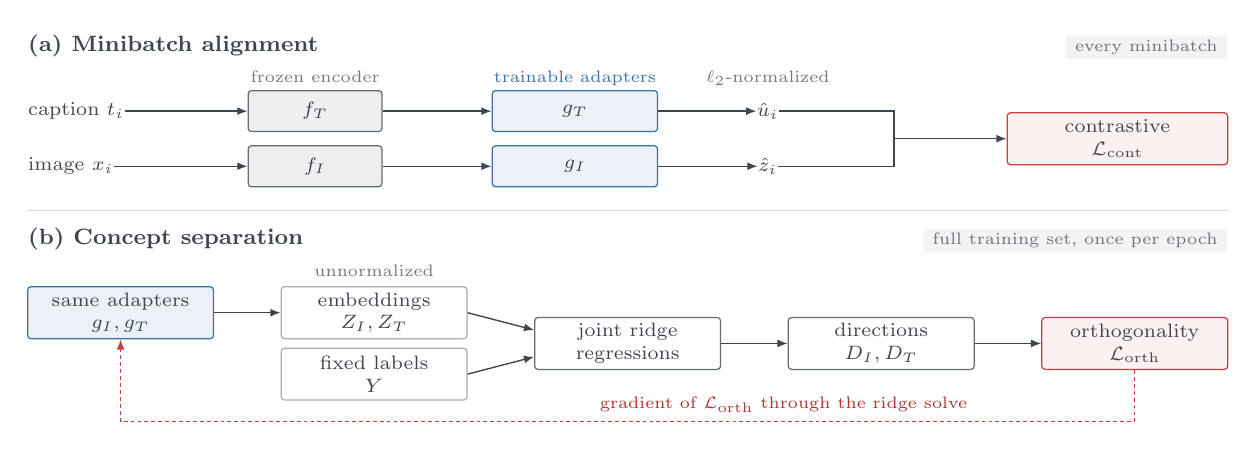
\begin{tikzpicture}[x=1mm, y=1mm]
  \useasboundingbox (0,0) rectangle (152.4,-51.0);

  % ---- (a) paired minibatch alignment ----------------------------------------
  \node[title] at (0,-3.0) {(a) Minibatch alignment};
  \node[tag] at (152.4,-3.0) {every minibatch};

  \node[header] at (36.5,-6.9) {frozen encoder};
  \node[header, text=roundblue] at (69.5,-6.9) {trainable adapters};
  \node[header] at (94.0,-6.9) {$\ell_2$-normalized};

  \node[plain, anchor=west] (t) at (0,-10.6) {caption $t_i$};
  \node[plain, anchor=west] (x) at (0,-17.6) {image $x_i$};
  \node[frozen, minimum width=17mm, minimum height=5.2mm] (fT) at (36.5,-10.6) {$f_T$};
  \node[frozen, minimum width=17mm, minimum height=5.2mm] (fI) at (36.5,-17.6) {$f_I$};
  \node[trained, minimum width=21mm, minimum height=5.2mm] (gT) at (69.5,-10.6) {$g_T$};
  \node[trained, minimum width=21mm, minimum height=5.2mm] (gI) at (69.5,-17.6) {$g_I$};
  \node[plain] (u) at (94.0,-10.6) {$\hat u_i$};
  \node[plain] (z) at (94.0,-17.6) {$\hat z_i$};
  \foreach \a/\b in {t/fT, fT/gT, gT/u, x/fI, fI/gI, gI/z}
    \draw[flow] (\a) -- (\b);

  \draw[joinline] (u.east) -- (110,-10.6) -- (110,-17.6) -- (z.east);
  \node[loss, minimum width=28mm, minimum height=6.6mm] (cont) at (138.4,-14.1)
    {contrastive\\$\mathcal{L}_{\mathrm{cont}}$};
  \draw[flow] (110,-14.1) -- (cont.west);

  \draw[divider] (0,-23.2) -- (152.4,-23.2);

  % ---- (b) full-training-set concept separation ------------------------------
  \node[title] at (0,-27.6) {(b) Concept separation};
  \node[tag] at (152.4,-27.6) {full training set, once per epoch};

  \node[header] at (44.0,-31.6) {unnormalized};

  \node[trained, minimum width=23.6mm, minimum height=6.6mm] (heads) at (11.8,-36.2)
    {same adapters\\$g_I, g_T$};
  \node[input, minimum width=23.6mm, minimum height=6.6mm] (Z) at (44.0,-36.2)
    {embeddings\\$Z_I, Z_T$};
  \node[input, minimum width=23.6mm, minimum height=6.6mm] (Y) at (44.0,-44.0)
    {fixed labels\\$Y$};
  \node[stage, minimum width=23.6mm, minimum height=6.6mm] (ridge) at (76.2,-40.1)
    {joint ridge\\regressions};
  \node[stage, minimum width=23.6mm, minimum height=6.6mm] (dirs) at (108.4,-40.1)
    {directions\\$D_I, D_T$};
  \node[loss, minimum width=23.6mm, minimum height=6.6mm] (orth) at (140.6,-40.1)
    {orthogonality\\$\mathcal{L}_{\mathrm{orth}}$};

  \draw[flow] (heads) -- (Z);
  \draw[flow] (Z.east) -- ([yshift=1.7mm]ridge.west);
  \draw[flow] (Y.east) -- ([yshift=-1.7mm]ridge.west);
  \draw[flow] (ridge) -- (dirs);
  \draw[flow] (dirs) -- (orth);

  % The orthogonality loss trains the adapters through the ridge solution.
  \draw[grad] (orth.south) -- (140.6,-50.0) -- (11.8,-50.0) -- (heads.south);
  \node[gradlabel] at (96.0,-48.4)
    {gradient of $\mathcal{L}_{\mathrm{orth}}$ through the ridge solve};
\end{tikzpicture}
\end{document}
